%摘要
\section*{Link Prediction}
Deep Bidirectional Language-Knowledge Graph Pretraining

%介绍
\section{论文摘要abstract和introduction翻译}

\subsection{论文摘要abstract翻译}
预训练的语言模型(LM)已经证明对各种下游NLP任务有帮助。最近的研究表明,知识图谱(KG)可以补充文本数据,提供结构化的背景知识,为推理提供有用的支撑。然而,这些研究还没有进行预训练,无法在大规模上学习这两种模式的深度融合,这限制了获取文本和KG完全联合表示的潜力。在这里,我们提出了 DRAGON(深度双向语言-知识图谱预训练),这是一种自我监督的方法,可以从大规模文本和KG中预训练深层联合语言-知识基础模型。具体来说,我们的模型将文本段和相关的KG子图作为输入,并双向融合来自两种模式的信息。我们通过统一两个自我监督的推理任务来预训练该模型,即掩码语言建模和KG链接预测。DRAGON在各种下游任务上优于现有的LM和LM+KG模型,包括跨一般和生物医学领域的问答任务,平均绝对增益为+5%。特别是,DRAGON 在涉及长上下文或多步骤推理的问题上表现出强大的性能(+10%),在低资源 QA 上(+8%在 OBQA 和 RiddleSense 上)以及各种 BioNLP 任务上取得了新的最先进的结果。我们的代码和训练模型可以在 https://github.com/michiyasunaga/dragon 上找到。

\subsection{论文introduction翻译}
从大量原始数据中得到的预训练学习自监督表示,可以帮助各种下游任务。在大量文本数据上进行预训练的语言模型(LMs),例如BERT和GPTs,在许多自然语言处理(NLP)任务中表现出色。这些模型的成功来自于通过自我监督大规模学习输入令牌的深度交互(情景化)表示。同时,大型知识图谱(KGs),如Freebase、Wikidata和ConceptNet,可以向文本数据提供补充信息。KG通过将实体表示为节点并将它们之间的关系表示为边缘来提供结构化的背景知识,还为结构化、多步骤推理实体提供了框架。文本数据和KG的双重优势激发了大规模预训练两个模态的深度交互表示的研究。

如何有效地将文本和知识图谱结合起来进行预训练是一个开放的问题,并且提出了挑战。对于文本和知识图谱,我们需要一个深层双向模型使两个模态进行交互,以及一个自我监督的目标以大规模对文本和知识图谱进行联合推理。现有的几项工作提出了自我监督预训练的方法,但它们以浅层或单向的方式融合文本和知识图谱。另一类工作提出了用于文本和知识图谱的双向模型,但这些模型侧重于在标记的下游任务上进行微调,而不是进行自我监督学习。因此,现有方法在建模和学习的深度交互方面可能有限制。

为了解决上述两个挑战并充分融合文本和知识图谱的优势,我们提出了DRAGON(深度双向语言-知识图谱预训练),这是一种从文本和知识图谱中进行深度双向、自我监督预训练语言知识模型的方法。DRAGON具有两个核心组件:一个跨模态模型,该模型以双向方式将文本和知识图谱作为输入,并学习两个模态之间的交互表示;以及一个双向自我监督目标,它通过最大化预测来自文本和知识图谱的跨模态掩码令牌的条件概率来学习联合推理。具体来说,如图1所示,我们采用一个文本语料库和一个知识图谱作为原始数据,并通过从文本语料库中采样一个文本段并从知识图谱中提取相关子图来为模型创建输入,从而获得(文本,本地知识图谱)对。我们使用跨模态模型将此输入编码为融合表示,其中模型的每个层用语言模型编码文本并用图神经网络编码知识图谱,并用双向模态交互模块(GreaseLM)将两者融合在一起。我们通过统一两个自我监督推理任务来预训练此模型:(1)掩码语言建模(MLM),该任务对输入文本中的令牌进行掩码和预测;(2)链接预测,该任务在输入知识图谱中丢弃和预测边缘。这样做的直觉是,通过结合这两个任务,MLM使模型将文本与结构化知识结合使用来进行文本中的掩码令牌推理(例如,在图1中,使用来自KG的“圆刷”-“艺术用品”多跳路径来帮助),链接预测使模型将知识图谱结构与文本上下文结合起来进行知识图谱中缺失链接的推理(例如,从文本中认识到“圆刷可用于头发”有助于这一点)。因此,这个联合目标使文本能够以知识图谱结构为基础,并使知识图谱能够以文本为背景同时进行情境化处理,从而产生一个深度统一的预训练语言知识模型,其中信息在文本和知识图谱之间进行双向流动以进行推理。

我们将在两个领域对DRAGON进行预训练:一是通用领域,使用Bookcorpus和ConceptNet KG;二是生物医学领域,使用PubMedcorpus和UMLSKG。我们发现,DRAGON在跨域的各种下游任务上优于现有的LM和LM + KG模型。对于一般领域,DRAGON在各种常识推理任务上,如CSQA、OBQA、RiddleSense和HellaSwag等,优于我们的基础LM RoBERTa,平均绝对准确率提高了8%。对于生物医学领域,DRAGON改进了之前的最佳LM BioLinkBERT,并为BioNLP任务设定了新的标准,如MedQA和PubMedQA,准确率提高了3%。特别的是,DRAGON在涉及复杂推理的QA任务上表现出明显的改进(在多步骤、否定、对冲或长上下文推理上提高了10%的准确率),在训练数据有限的下游任务上也有所提高(提高了8%的准确率)。这些结果表明,与现有模型相比,我们对文本和KG进行深度双向自我监督所产生的语言知识表示有了显著改进。

知识增强LM预训练。知识集成是改进LM的积极研究方向。一条工作线是检索增强LMs,它从语料检索相关文本,并将其作为附加知识集成到LMs中。与这些作品正交,我们专注于使用知识库作为背景知识,对实体和事实进行基础推理。

与我们的工作最相关的是将知识库集成到LM预训练中的工作。其中一项研究旨在向LM添加实体特征;一些工作使用KG实体信息或结构来创建额外的训练信号;一些工作将KG三元组信息直接添加到LM的输入中。虽然这些方法取得了重大进展,但它们通常以浅层或单向(例如,KG到文本)的方式在文本和KG之间传递信息,这可能限制了完全联合推理两个模态的潜力。为了改进上述方法,我们提出通过深度跨模态模型和联合自我监督来双向交互文本和KG,使文本和KG相互接地和情境化。我们发现这可以改善模型在各种推理任务上的性能(第3节)。另一个区别是,这个领域中的现有工作通常侧重于从KG中添加实体或三元组级别的知识到LM中,并专注于解决实体/关系分类任务。我们的工作显著扩大了这个范围,因为我们使用更大的KG子图(200个节点)作为输入,以在KG和文本之间实现更丰富的情境化,我们在包括QA、推理和文本分类任务在内的更广泛的NLP任务上实现了性能提升。

知识图谱增强问答。各种工作设计了KG增强的推理模型用于问答。特别是最近的工作,如QA-GNN和GreaseLM ,表明知识图谱可以通过其图结构来支撑对实体的推理,并有助于复杂的问题解答(例如,否定,多跳推理)。这些工作通常侧重于在特定的QA数据集上训练或微调模型。相比之下,我们对此进行了泛化并将KG增强的推理集成到通用预训练中。我们的动机是自监督预训练允许模型从更大型和更多样化的数据中学习,这有助于学习文本与KG之间更丰富的交互,并获得超越特定QA任务的更多样化的推理能力。我们发现我们的预训练方法(DRAGON)对各种下游任务的基线QA模型(例如GreaseLM)提供了显著的推动力。这开辟了一个新的研究途径,将各种精心设计的QA模型扩展到预训练。

知识图谱表示学习。我们在预训练中使用的链接预测任务受到知识图谱表示学习的研究启发。链接预测是知识图谱的基本任务,各种工作研究学习KG实体和关系嵌入的方法用于链接预测,例如TransE,DistMult 和RotatE。一些作品还使用文本数据或预训练的LM来帮助学习KG嵌入和链接预测。虽然这些作品关注KG一侧的表示,但我们将范围扩展到使用KG一侧的目标(链接预测)与文本侧的目标(语言建模)联合训练相互交互的文本-KG模型。

\section{问题描述}
文本预训练在许多NLP任务中表现出色,同时,大型知识图谱(KGs)可以向文本数据提供补充信息,为实体间的关系提供结构化的背景知识。如何有效地将文本和知识图谱结合起来进行预训练是一个开放的问题。现有的工作要么研究的方向不是预训练,要么侧重于在标记的下游任务上进行微调。为了这个挑战并充分融合文本和知识图谱的优势,作者提出了DRAGON模型,深度双向语言-知识图谱预训练。

\section{输入、输出、模型算法描述}
\subsection{输入}
在预训练中,输入的是文本数据和知识图谱
\subsection{输出}
在预训练中,输出的是文本——知识图谱对,以及模型的损失函数
\subsection{模型算法描述}
初始化模型参数。

对于每个预训练步骤,执行以下操作:
从数据集中随机采样一个联合文本-知识图谱对。
对于每个文本令牌wi,以15%的概率将其替换为[MASK]特殊令牌。
执行掩码语言建模任务,使用上下文化令牌向量{Hi}和特殊令牌[MASK]来预测原始令牌{wi}。
执行知识图谱链接预测任务,保留输入知识图谱中的一些边缘并预测它们。
计算模型的损失函数,包括掩码语言建模损失和知识图谱链接预测损失。
使用反向传播算法更新模型的参数。
如果达到了指定的训练步数或验证集性能指标,则终止预训练过程。

使用预训练的模型进行下游任务。
\begin{figure}[H]
  \centering
  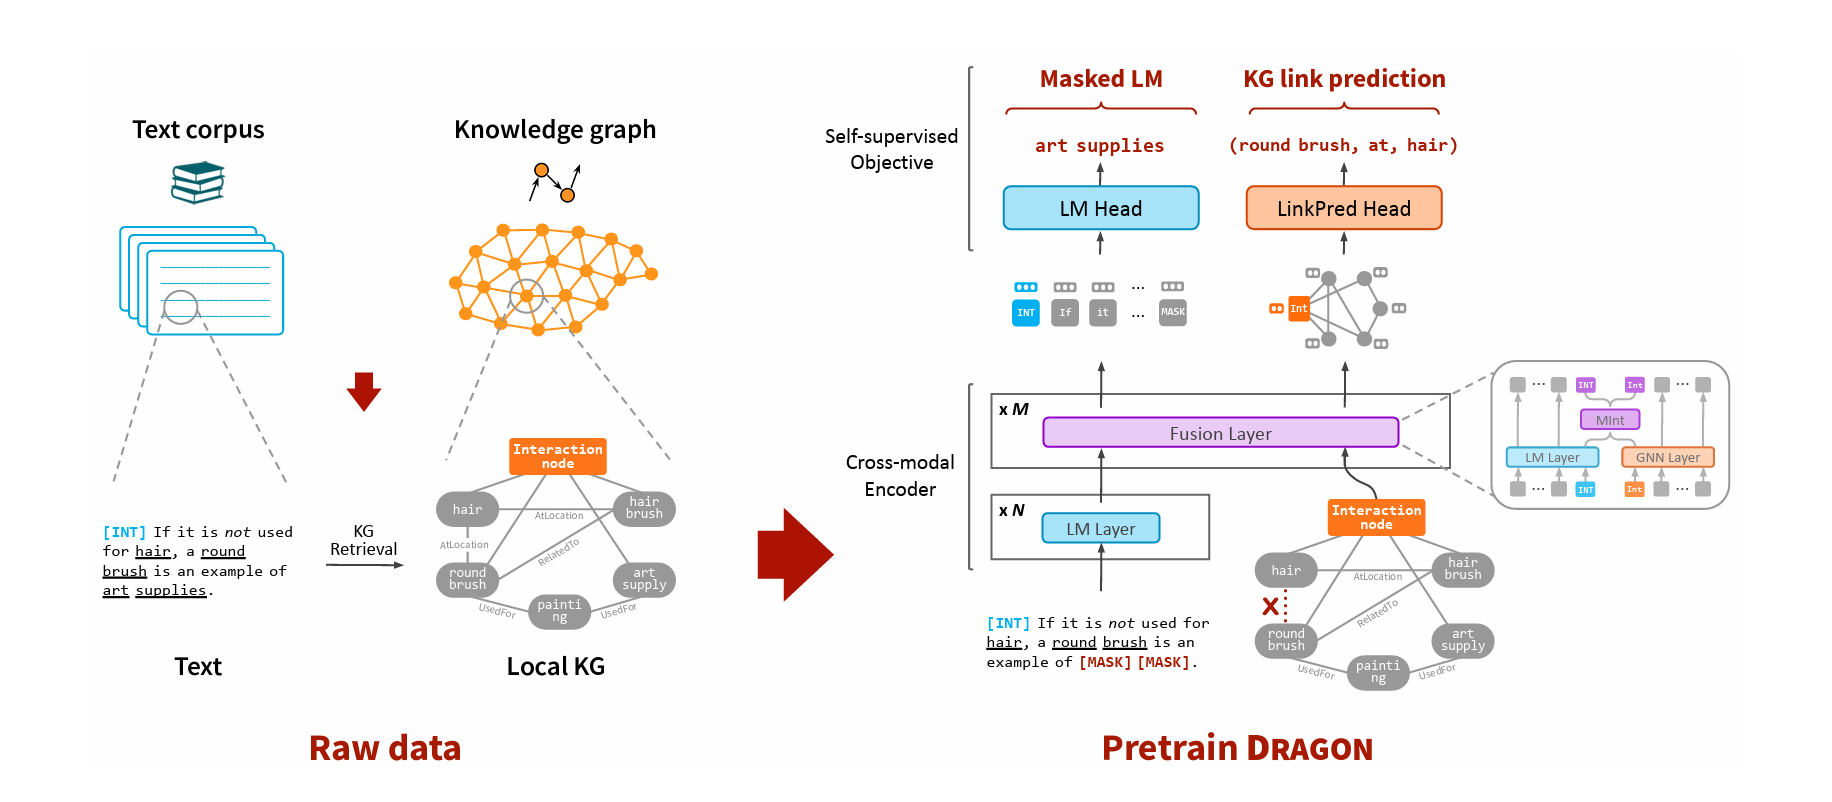
\includegraphics[width=\textwidth]{figure/1.png}
  \caption{}
  \label{fig:my_label}
\end{figure}

\subsection{评价指标及其计算公式}
作者使用了两个子监督推理任务,MLM和Link prediction。两个任务各自有自己的损失函数。作者讲两个损失函数集合起来,给出了一个评价函数
\begin{figure}[H]
  \centering
  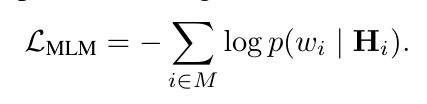
\includegraphics[width=\textwidth]{figure/2.png}
  \caption{}
  \label{fig:my_label}
\end{figure}
\begin{figure}[H]
  \centering
  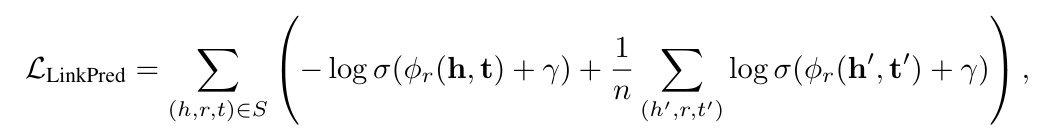
\includegraphics[width=\textwidth]{figure/3.png}
  \caption{}
  \label{fig:my_label}
\end{figure}
\begin{figure}[H]
  \centering
  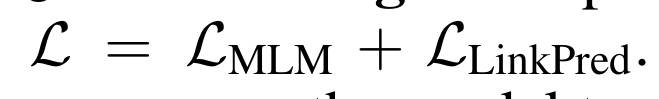
\includegraphics[width=\textwidth]{figure/4.png}
  \caption{}
  \label{fig:my_label}
\end{figure}


\section{对比方法及这些对比方法的引用论文出处}
\subsection{对比方法}
RoBERTa QAGNN GreaseLm
\subsection{对比方法的引用论文出处}
RoBERTa:  Yinhan Liu, Myle Ott, Naman Goyal, Jingfei Du, Mandar Joshi, Danqi Chen, Omer Levy, Mike Lewis, Luke Zettlemoyer, and Veselin Stoyanov. Roberta: Arobustly optimized bert pretraining approach. arXiv preprint arXiv:1907.11692, 2019.

QAGNN:  Michihiro Yasunaga, Hongyu Ren, Antoine Bosselut, Percy Liang, and Jure Leskovec. QAGNN: Reasoning with language models and knowledge graphs for question answering. In NorthAmerican Chapter ofthe Association for Computational Linguistics(NAACL), 2021.

GreaseLm: XikunZhang, Antoine Bosselut, Michihiro Yasunaga, Hongyu Ren, Percy Liang, Christopher DManning, and Jure Leskovec. Greaselm: Graph reasoning enhanced language models forquestion answering. In International Conference on Learning Representations(ICLR), 2022

\section{结果}
作者一共提供了四个数据集,在train的过程中,前三个数据集都取得了和论文中一致的结果,但是第四个数据集并未取得和论文中相近的结果。由于在租用的3090服务器上,第四个数据集的train需要20多小时,没有足够时间再进行训练去排查问题可能所在。我们在前三个数据集的训练中,看到了和论文中十分接近的结果。

以下展示wandb网站截图和输出文件截图。完整的输出、log、json文件都在代码train文件夹中
\begin{figure}[H]
  \centering
  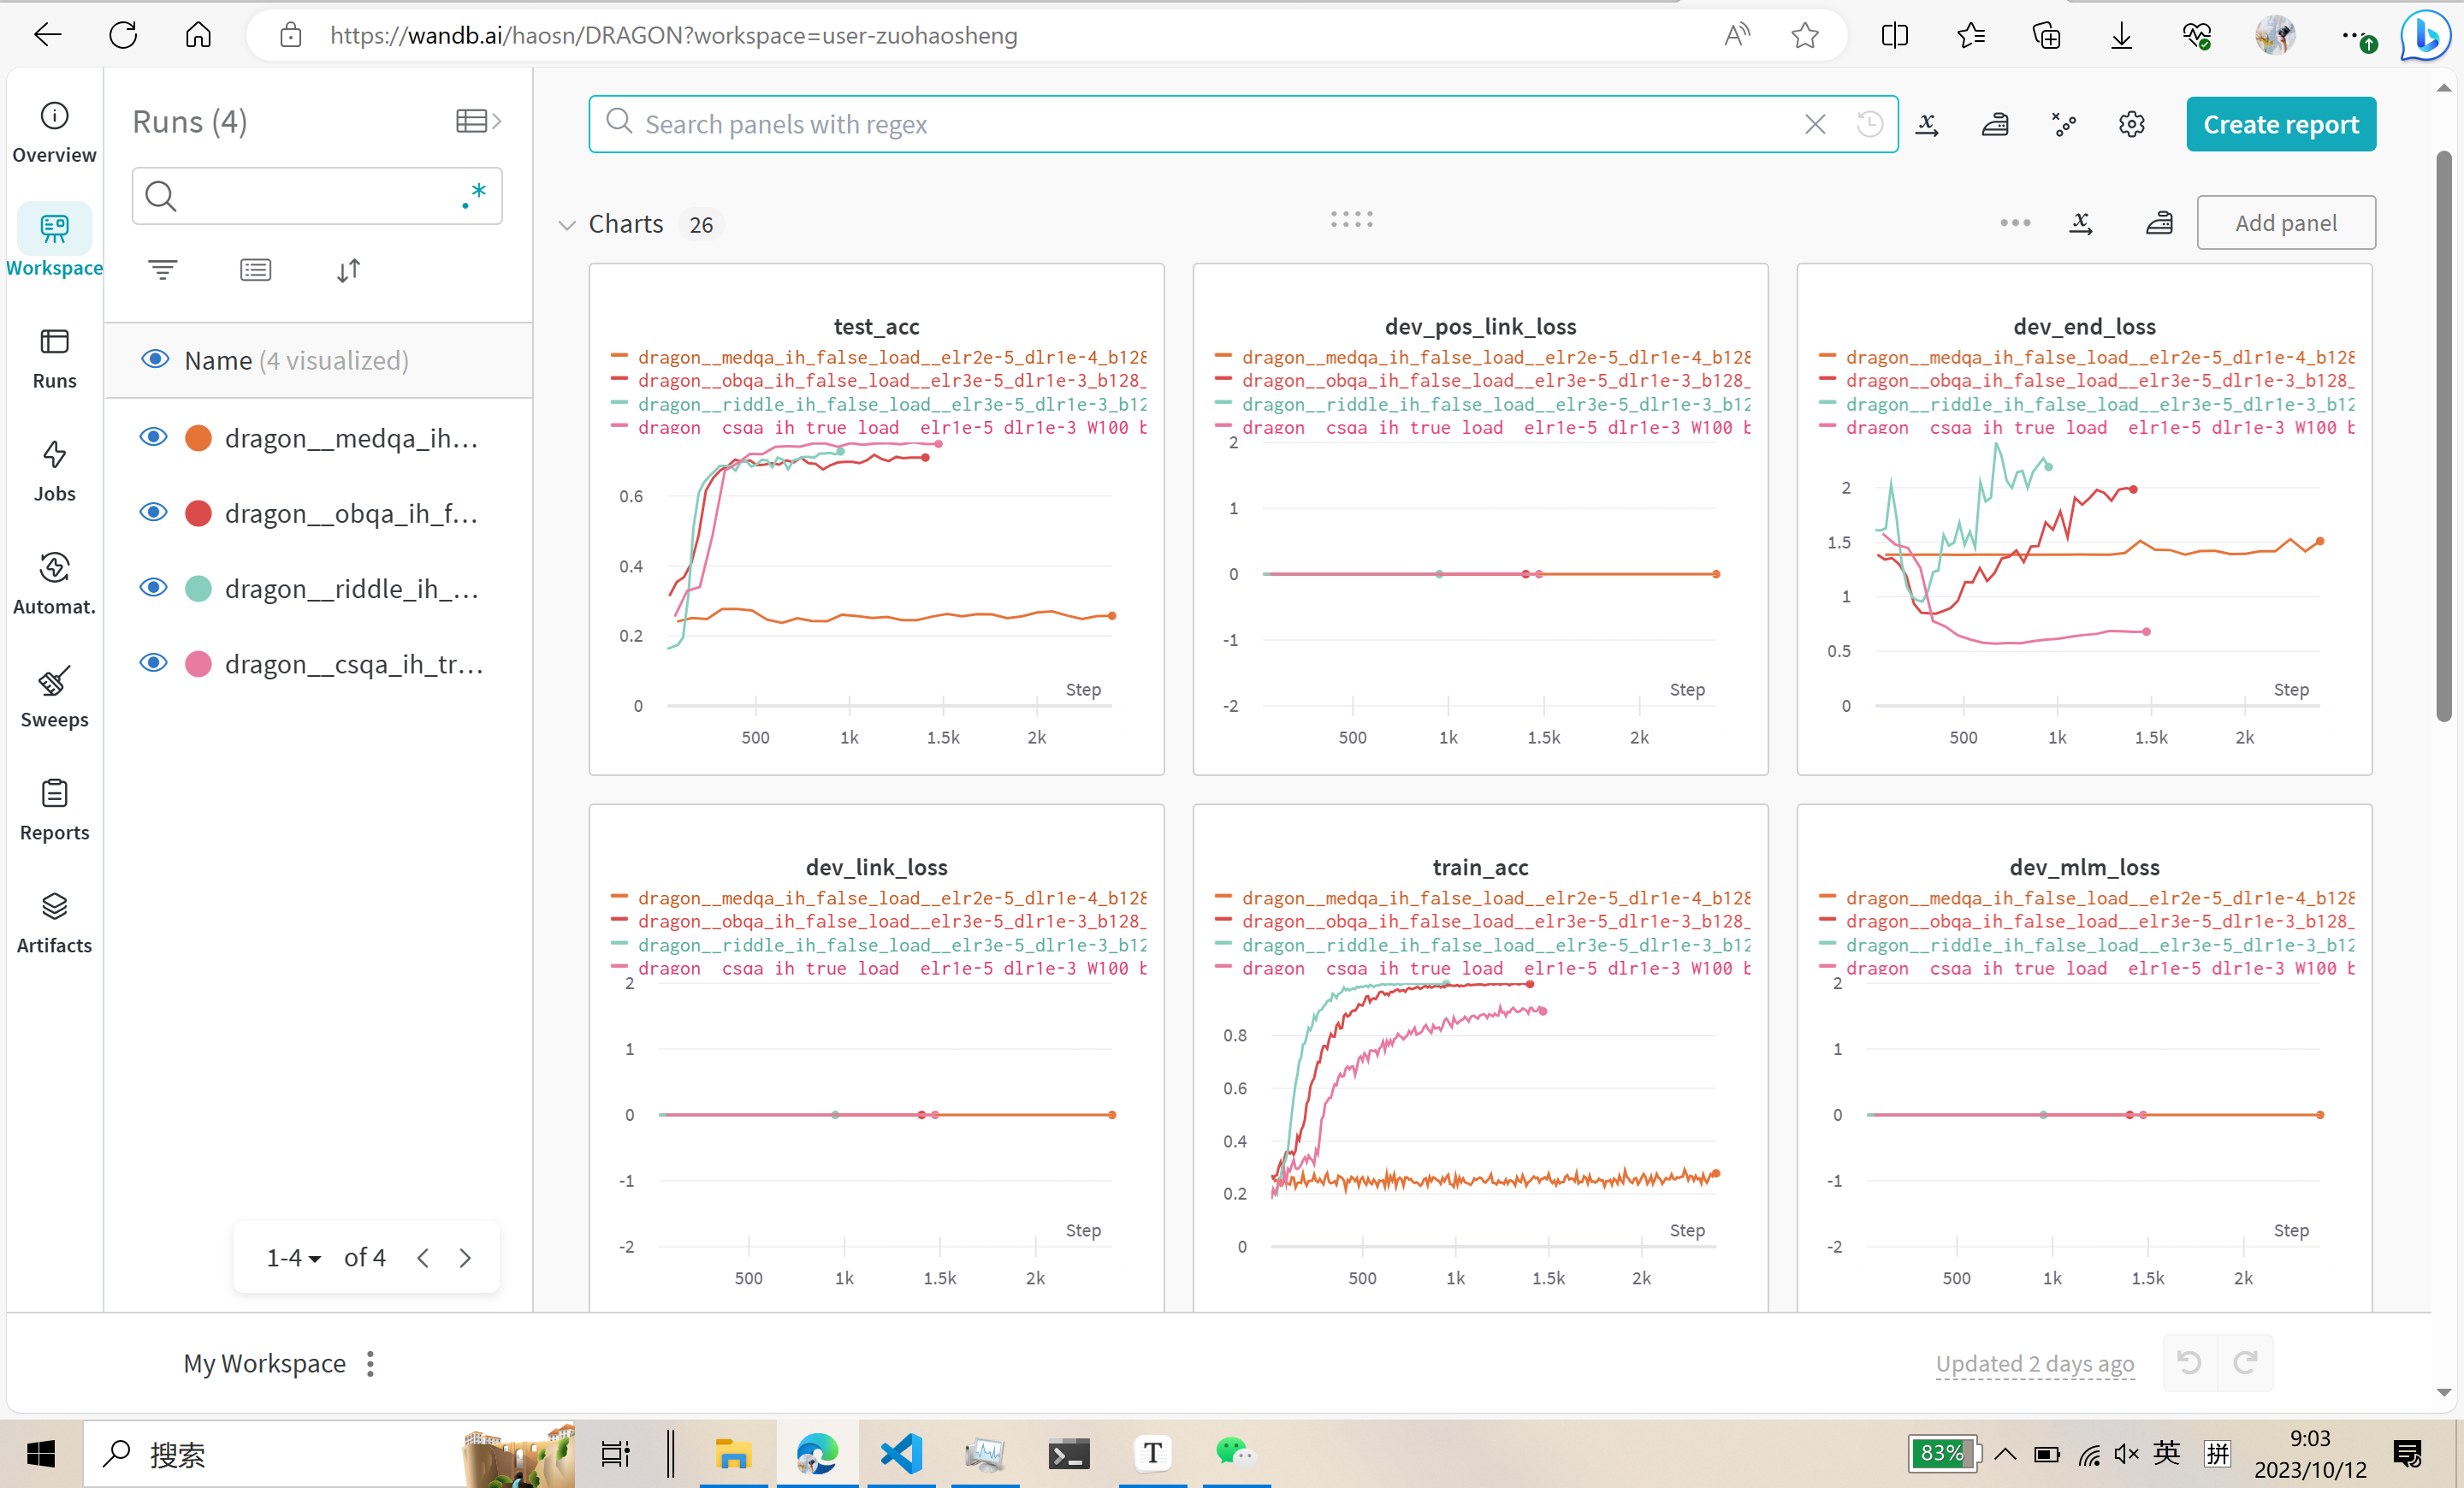
\includegraphics[width=\textwidth]{figure/5.png}
  \caption{}
  \label{fig:my_label}
\end{figure}
\begin{figure}[H]
  \centering
  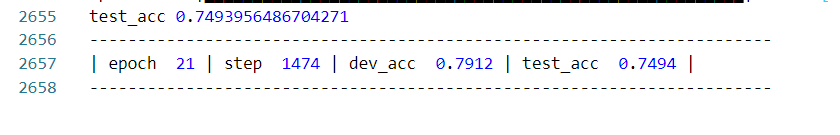
\includegraphics[width=\textwidth]{figure/csqa.png}
  \caption{csqa}
  \label{fig:my_label}
\end{figure}
\begin{figure}[H]
  \centering
  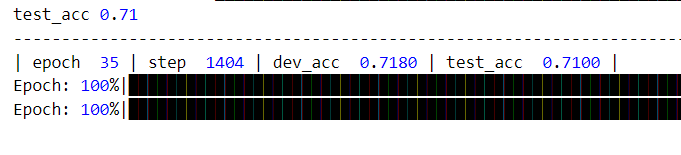
\includegraphics[width=\textwidth]{figure/obqa.png}
  \caption{obqa}
  \label{fig:my_label}
\end{figure}
\begin{figure}[H]
  \centering
  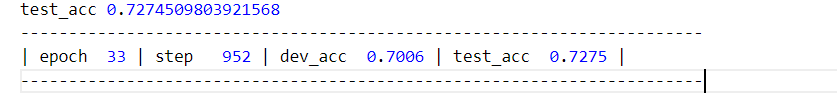
\includegraphics[width=\textwidth]{figure/riddle.png}
  \caption{riddle}
  \label{fig:my_label}
\end{figure}
\begin{figure}[H]
  \centering
  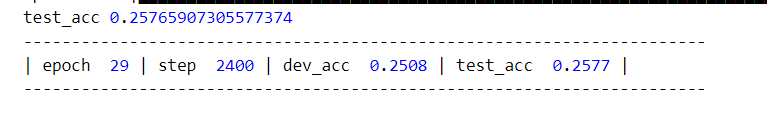
\includegraphics[width=\textwidth]{figure/medqa.png}
  \caption{medqa}
  \label{fig:my_label}
\end{figure}

对于作者提供的训练好的模型,进行下载检验准确度,获得结果和论文中结果一致

以下为部分控制台输出截图,完整截图在代码eva文件夹中
\begin{figure}[H]
  \centering
  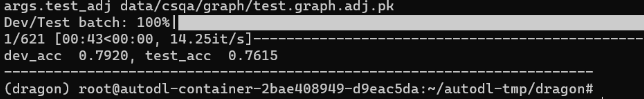
\includegraphics[width=\textwidth]{figure/csqa1.png}
  \caption{csqa}
  \label{fig:my_label}
\end{figure}
\begin{figure}[H]
  \centering
  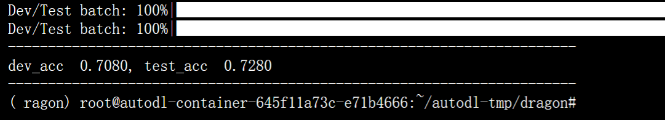
\includegraphics[width=\textwidth]{figure/obqa1.png}
  \caption{obqa}
  \label{fig:my_label}
\end{figure}
\begin{figure}[H]
  \centering
  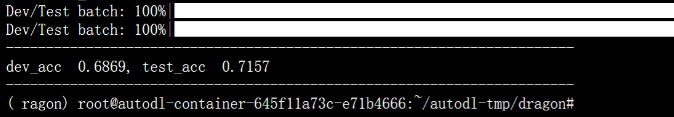
\includegraphics[width=\textwidth]{figure/riddle1.png}
  \caption{riddle}
  \label{fig:my_label}
\end{figure}
\begin{figure}[H]
  \centering
  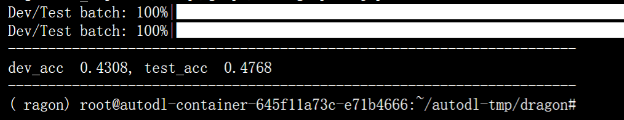
\includegraphics[width=\textwidth]{figure/medqa1.png}
  \caption{medqa}
  \label{fig:my_label}
\end{figure}